%\documentclass[border=3mm]{standalone}
%\usepackage{pgfplots}
%\pgfplotsset{compat=newest}
%\pagestyle{empty}
%\begin{document}
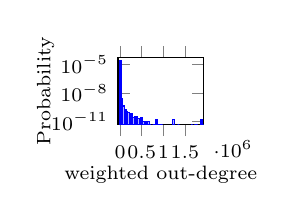
\begin{tikzpicture}
\begin{axis}[ymax=0.00005,ybar,ymode=log,bar width=38609.75576939172,log origin=infty,xmin=-50000.75576939172,enlargelimits=0,
width=.22\textwidth,
height=.20\textwidth,
ylabel=Probability,
xlabel=weighted out-degree,
every axis y label/.append style={
      yshift=-8pt,
    },
every axis x label/.append style={
      yshift=4pt,
    },
every x tick scale label/.style={at={(xticklabel cs:1)},anchor=south west},
  label style={font=\scriptsize},
tick label style={font=\scriptsize} ,
]
\addplot  plot coordinates {
(0.0, 2.58962633811e-05)
(38609.7557694, 2.74085967219e-09)
(77219.5115388, 4.17293514104e-10)
(115829.267308, 1.75452954794e-10)
(154439.023078, 1.13807322028e-10)
(193048.778847, 8.53554915214e-11)
(231658.534616, 6.16456327654e-11)
(270268.290386, 6.63876045166e-11)
(308878.046155, 2.37098587559e-11)
(347487.801925, 2.84518305071e-11)
(386097.557694, 2.84518305071e-11)
(424707.313463, 1.89678870047e-11)
(463317.069233, 9.48394350237e-12)
(501926.825002, 2.37098587559e-11)
(540536.580771, 9.48394350237e-12)
(579146.336541, 9.48394350237e-12)
(617756.09231, 9.48394350237e-12)
(656365.84808, 9.48394350237e-12)
(694975.603849, 4.74197175119e-12)
(733585.359618, 0.0)
(772195.115388, 4.74197175119e-12)
(810804.871157, 4.74197175119e-12)
(849414.626927, 1.42259152536e-11)
(888024.382696, 4.74197175119e-12)
(926634.138465, 4.74197175119e-12)
(965243.894235, 4.74197175119e-12)
(1003853.65, 0.0)
(1042463.40577, 0.0)
(1081073.16154, 0.0)
(1119682.91731, 0.0)
(1158292.67308, 0.0)
(1196902.42885, 0.0)
(1235512.18462, 1.42259152536e-11)
(1274121.94039, 0.0)
(1312731.69616, 0.0)
(1351341.45193, 4.74197175119e-12)
(1389951.2077, 0.0)
(1428560.96347, 0.0)
(1467170.71924, 0.0)
(1505780.47501, 0.0)
(1544390.23078, 0.0)
(1582999.98655, 0.0)
(1621609.74231, 0.0)
(1660219.49808, 4.74197175119e-12)
(1698829.25385, 0.0)
(1737439.00962, 4.74197175119e-12)
(1776048.76539, 4.74197175119e-12)
(1814658.52116, 0.0)
(1853268.27693, 0.0)
(1891878.0327, 1.42259152536e-11)
(1930487.78847, 4.74197175119e-12)
};\end{axis}
\end{tikzpicture}
%\end{document}
